%!TEX root = paper.tex

\section{Introduction} % (fold)
\label{sec:introduction}
Automatic loop invariant generation is fundamental for program analysis. A loop invariant can be useful for software verification, compiler optimization, program understanding, etc. In the following, we first define the loop invariant generation problem and then briefly mention existing approaches and then our proposal. For simplicity, we assume that we are given a Hoare triple in the following form:
%\[
%    P = \{ \mathit{Pre} \} \mathit{while}(\mathit{Cond}) \{ \mathit{Body} \} \{ \mathit{Post} \}
%\]
\begin{align*}
&\{Pre\} & & /\star\text{\emph{Assumption}}\star/ \\
&while (Cond) \{ Body \} && /\star\text{\emph{Loop Body}}\star/\\
&\{Post\} & & /\star\text{\emph{Assertion}}\star/
\end{align*}
Assume that $V = \{x_1{,} x_2{,} \cdots{,} x_n\}$ is a finite set of program variables which are relevant to the loop body. $Pre$, $Cond$ and $Post$ are predicates constituted by variables in $V$.
%In practice, the pre-condition $\mathit{Pre}$ is often described by
%the specification documents and checking conditions of the program inputs,
%and the post-condition $\mathit{Post}$ is usually specified
%by assertions and exceptions leading to an error state in the program.
Let $s = \{ x_1 \mapsto v_1, \ldots, x_n \mapsto v_n \}$ be a valuation of $V$. Let $\phi$ be a predicate constituted by variables in $V$. We write $s \models \phi$ to denote that $\phi$ valuates to true given the program state $s$. We write $s \not \models \phi$ otherwise.
$\mathit{Body}$ is an imperative program which updates the valuation of $V$. For simplicity, we assume that it is a deterministic function on valuations of variables $V$, and write $\mathit{Body}(s)$ to denote the valuation of $V$ after executing $\mathit{Body}$ \LJ{from the} variable valuation $s$. For convenience, $\mathit{Body}^i(s)$ where $i \geq 0$ is defined as follows: $\mathit{Body}^0(s) = s$ and $\mathit{Body}^{i+1}(s) = \mathit{Body}(\mathit{Body}^i(s))$.
%the evaluation function of the program variables $x_1, \ldots, x_n$
%and $\mathit{Body}(s)$ stand for their new evaluation after the execution of $\mathit{Body}$,
%the above program means that (1) $\mathit{Pre}$ is the assumption to the initial value of $s$;
%(2) if the $\mathit{Cond}$ is satisfied by $s$ at an iteration,
%$\mathit{Body}$ will be executed and $s$ will be updated to $\mathit{body}(s)$;
%(3) if the $\mathit{Cond}$ is unsatisfied by $s$ at an iteration,
%the while-loop ends and $s$ should satisfy $\mathit{Post}$.

In order to prove the Hoare triple, we would like to find a loop invariant $\mathit{Inv}$ which satisfies the following three conditions.
\begin{align}
    &s \models \mathit{Pre}
        &&\Longrightarrow & s &\models \mathit{Inv} \label{inv:pre} \\
    &s \models \mathit{Inv} \wedge \mathit{Cond}
        &&\Longrightarrow & \mathit{Body}(s) &\models \mathit{Inv} \label{inv:loop} \\
    &s \models \mathit{Inv} \wedge \neg \mathit{Cond}
        &&\Longrightarrow & s &\models \mathit{Post} \label{inv:post}
\end{align}
Alternatively, we would like to find a valuation $s$ such that $s \models \mathit{Pre}$ and executing the loop until it terminates results in a valuation $s'$ such that $s' \not \models Post$.
The problem is thus either to prove the Hoare triple (by identifying an $\mathit{Inv}$ satisfying the three conditions) or to disprove it (by finding a valuation $s$ as described above). For simplicity, we further assume that the loop body always terminates and refer the readers to~ \cite{Domagoj:FAC:2013,LeQC:PLDI:15,Hong:ASE:2015} %%\cite{acmcomm}
 for an introduction on extensive research on proving loop termination.

Many approaches have been proposed for invariant generation. 
For example, there are proposals based on abstraction interpretation~\cite{cousot1978automatic,mine2006octagon,cousot1979systematic,karr1976affine,vincent2009subpolyhedra}, counterexample guided abstraction refinement~\cite{henzinger2003software,thomas2001slam,edmund2003counterexample}, interpolation~\cite{kenneth2010lazy,thomas2004abstractions,kenneth2003interpolation,Kenneth2006lazy} and constraint solving and inference~\cite{ashutosh2009invgen,michael2003linear,sumit2009constraint}. 
Recently, the authors of~\cite{sharma2012interpolants,sharma2013verification,sharma2014invariant} proposed to automatically generate loop invariants based on random searching~\cite{sharma2014invariant} as well as machine learning~\cite{sharma2012interpolants}. 
Their approaches start with randomly generating valuations of $V$, executing the program and collecting variable valuations after each iteration of the loop (a.k.a.~the samples). 
Since by definition these samples must satisfy the loop invariant $\mathit{Inv}$ (if there is any), machine learning techniques are used to generalize them in certain form to obtain candidate loop invariants. 
For instance, classification algorithms like Support Vector Machines (SVM) ~\cite{sharma2012interpolants,sharma2013verification} can be used to generate classifiers as candidate invariants. 
The candidates are then checked using program verification techniques (like symbolic execution~\cite{symbolic}) to see whether they satisfy the three conditions. If certain condition is violated, we obtain counterexamples in the form of variable valuations. 
For instance, having a candidate $C$, if condition (1) is violated, a valuation $s$ satisfying $s \models Pre \land s \not \models C$ is generated, which \LJ{proves $C$ is not an actual invariant}. 
With this new sample, we can apply the classification algorithm again to obtain a new candidate invariant. The learn-and-check iteration is repeated until an invariant satisfying the conditions are identified or a valuation disproving the Hoare triple is.

One problem of the above approach is that its effectiveness is often limited by the samples which are generated either randomly or through verification. In order to learn the right invariant through classification, often a large number of samples are necessary. Furthermore, often we must have those samples right by the boundary between variable valuations which satisfy the actual invariant and those which do not, so that classification techniques would identify the right invariant. Obtaining those samples through random sampling is often hard. As a result, many iterations of learn-and-check are necessary before the candidate invariant converges to the right one. Another problem is that the loop invariants obtained through existing learn-and-check approaches~\cite{sharma2012interpolants,sharma2013verification,sharma2014invariant} are limited to linear inequalities or their conjunctions.

In this work, we propose a framework for loop invariant generation following the same learn-and-check approach. %We improve existing approaches in two aspects. First, by adopting active learning techniques, we improve the quality of the candidate invariants prior to verifying them, in every iteration of learn-and-check. As a result, we can reduce the number of learn-and-check iterations significantly. Second, by supporting an extensible framework, we can easily integrate different classification techniques (e.g., SVM with kernel methods~\cite{}) as well as the corresponding active learning techniques so that we can learn a large class of invariants. %We have developed a prototype implementation of our method and applied to benchmark programs including those from the software verification competition. The results show that our method often reduces the number of guess-and-check iterations as well as is able to learning more loop invariants than existing approaches.
%In the following, we define our problem and briefly illustrate how our approach works.
Compared to the existing approaches, we make the following contributions. Firstly, we propose to adopt active learning techniques to (partially) overcome the limitation of random sampling. That is, active learning allows us to automatically generate samples which are important in improving the quality of the candidate invariants so that we can improve the candidates prior to verifying them during every learn-and-check iteration. As a result, we can reduce the number of learn-and-check iterations significantly.
%    for automatic invariant inference based on machine learning.
%    Since the samples are chosen for clear purpose
%    to refine the invariant candidate in the \emph{data collection} stage,
%    the invariant converges efficiently.
%    Furthermore, because the counter-examples generated in the \emph{invariant verification} stage
%    give very accurate information to amend the invariant candidate,
%    they become a useful supplementary to overcome the weakness of machine learning
%    and fine-tune the invariant candidate.
Secondly, \LJ{our framework is designed to be} extensible to different learning algorithms. For instance, we show that we can easily extend our framework to learn candidate invariants in the form of polynomial inequalities or their conjunctions.
Lastly, we implement our framework as a tool called \textsc{Zilu}
    and compare it with other available state-of-the-art invariant inference tools,
    i.e., CPAChecker~\cite{beyer2011cpachecker} and Interproc~\cite{jeannet2010interproc}.
%    Our experiment results show that
%    we are the only tool that can work with polynomial invariant inference.
%    Notice that the polynomial invariant inference works in our framework
%    naturally with very light additional programming.
    % Based on the design of different approaches,
    % we also claim that our framework have better extensibility comparing with their method.
    \textsc{Zilu} is built upon existing tools (e.g., GNU Scientific Library (GSL)~\cite{gough2009gnu} for selective sampling,
    LibSVM~\cite{chang2011libsvm} for SVM classification,
    revised KLEE~\cite{cadar2008klee} for symbolic execution~\cite{king1976symbolic,symbolic}, and Z3~\cite{de2008z3} for invariant verification) and can be used as a language/platform independent tool to verify programs.

\paragraph{Organization} The remainders of the paper are organized as follows. Section~\ref{sec:overview} presents an overview of our approach using an illustrative example. Section~\ref{sec:sampling} and~\ref{sec:learning} then presents details on two main steps in our framework: data collection and active learning. Section~\ref{sec:evaluations} discusses our prototype implementation and evaluates its effectiveness using a set of benchmark programs. Section~\ref{sec:related} reviews related work and concludes.

\section{Overview through an Example} \label{sec:overview}
In our framework, loop invariant generation is an iterative process of \emph{data collection}, \emph{active learning} and \emph{candidate verification}. The overall workflow is shown in the Figure~\ref{fig:overview}. In the following, we use a simple example to illustrate how our approach works.

\begin{figure}[t]
    \centering
    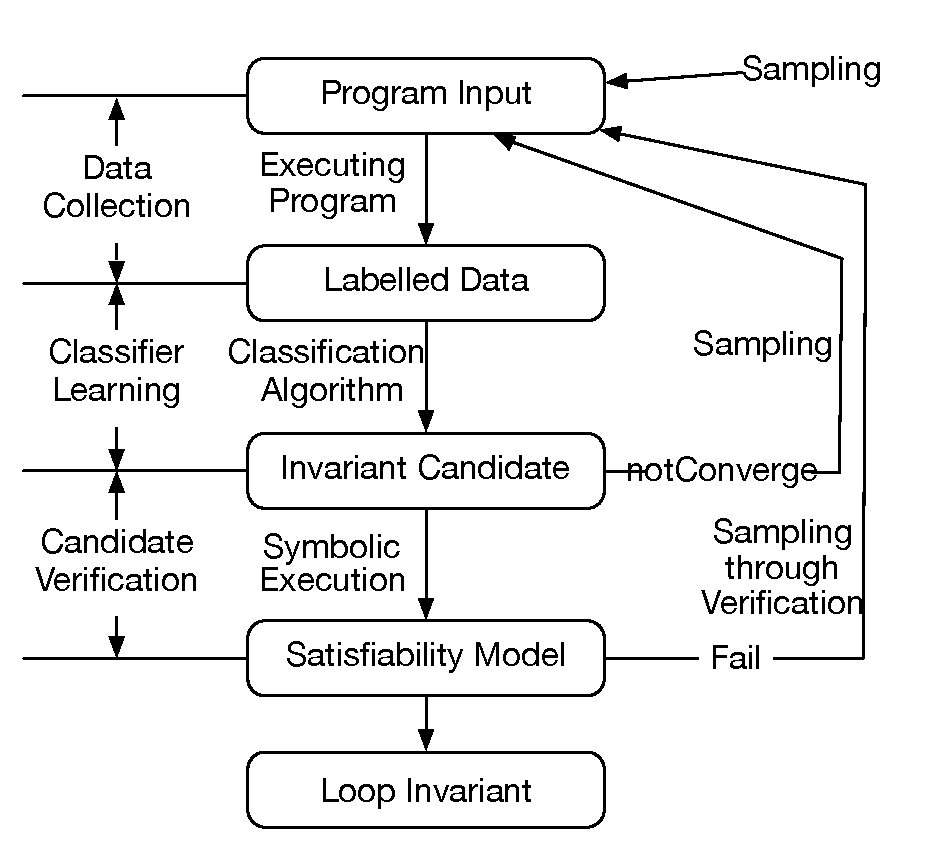
\includegraphics[scale=0.45]{figures/overview.pdf}
    \caption{Loop Invariant Inference Framework Overview}
    \label{fig:overview}
\end{figure}

\begin{figure}[t]
\begin{subfigure}{0.5\textwidth}
    \raggedright
    \vspace{0.5cm}
%% {\scriptsize\begin{verbatim}
%% void P(int x, int y) {
%%     assume(x < y);
%%     while (x < y) {
%%         if (x < 0) x = x + 7;
%%         else x = x + 10;

%%         if (y < 0) y = y - 10;
%%         else y = y + 3;
%%     }
%%     assert(x >= y
%%         && x <= y + 16);
%% }
%% \end{verbatim}}
\vspace{-0.2cm} \[
 \begin{array}{ll}
1 & \code{void~P(int ~x{,} ~int~y)\{} \\
2 & \code{~~~ assume(x~{<}~y);}  \\
3 & \code{~~~ while(x~{<}~y)\{}  \\
4 & \code{~~~ \quad if~(x~{<}~0)~x~{=}~x~{+}~7;}  \\
5 & \code{~~~ \quad else~ x~{=}~x~{+}~10;}\\
6 & \code{~~~ \quad if~(y~{<}~0)~y~{=}~y~{-}~10;} \\
7 & \code{~~~ \quad else~ y~{=}~y~{+}~3;}\\
8 & \code{~~~\}} \\
9 & \code{~~~assert(x~{\geq}~y}\\
10 & \code{~~~\quad \&\&~x~{\leq}~y~{+}~16);}\\
11  & \}
\end{array}
\]
    \vspace{-0.2cm}
    \caption{A sample program}
    \label{fig:running:example:program}
\end{subfigure}%
\begin{subfigure}{.5\textwidth}
      \centering
      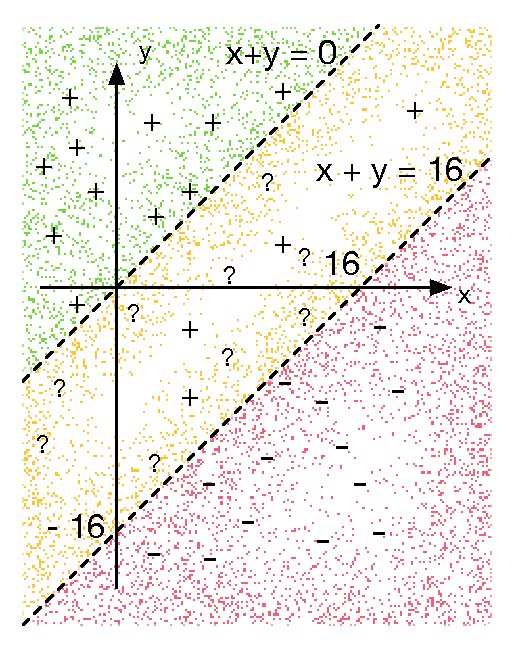
\includegraphics[scale=0.42]{figures/running-sampling.pdf}
      \caption{Sampling}
      \label{fig:running:example:sampling}
\end{subfigure}
\caption{A running example}
\label{fig:running:example}
\end{figure}
%%%sunjun: the two lines should x - y = 0 and x - y = 16.


\begin{example}
An example Hoare triple is shown in Figure~\ref{fig:running:example:program} (where an \code{assume} statement captures the precondition and an \code{assert} statement captures the postcondition). The set of variables $V$ contains two integer-type ones: $x$ and $y$. For simplicity, we interpret integers in the programs as mathematical integers (i.e., they do not overflow). The precondition $Pre$ is $x < y$, which is the same as the loop condition $Cond$.
During each loop iteration, $x$ is increased by $7$ if it is negative (line 4); otherwise it is increased by $10$ (line 5). $y$ is decreased by $10$ if it is negative (line 6); otherwise it is increased by $3$ (line 7). The postcondition $Post$ is $y \le x \le y + 16$. It is easy to check that the Hoare triple can be proven using a loop invariant $Inv$: $x \le y + 16$. In the following, we show how our framework works to learn this loop invariant.
\end{example}
We start with \emph{data collection}. Given the Hoare triple, we first randomly generate a set of valuations of $V$. For instance, we can adopt a constraint solver to generate random valuations which satisfy or fail $Pre$ as random samples. For each sample $s_0$ (i.e., a variable valuation), we execute the given program with the initial state $s_0$ and record the variable evaluations after each iteration of the loop. %as a trace $\langle s_0, s_1, \ldots, s_n \rangle$ where $s_n \not \models Cond$. Let $T$ denote the set of traces. We write $s \Rightarrow_T s'$ to denote that there exists a trace $\langle s_0, s_1, \cdots, s, \cdots, s', \cdots, s_n \rangle \in T$.
Let $Inv$ denote any invariant which satisfies condition (1), (2) and (3.) All variable valuations are then divided into four categories.
\begin{itemize}
    \item Set $\mathit{CE}$ contains the set of valuations which satisfy the precondition and violate the postcondition afterwards. We remark that anytime a valuation in $\mathit{CE}$ is identified, a counterexample is found and the Hoare triple is falsified.
    \item Set $\mathit{Positive}$ contains the set of valuations which satisfy the precondition and the postcondition afterwards. In Section~\ref{sec:sampling}, we show that every valuation in $\mathit{Positive}$ must satisfy $Inv$.
    \item Set $\mathit{Negative}$ contains the set of valuations which neither satisfy the precondition nor the postcondition afterwards. In Section~\ref{sec:sampling}, we show that every valuation in $\mathit{Negative}$ must fail $Inv$.
    \item Set $\mathit{NP}$ contains the set of valuations which do not satisfy the precondition but satisfy the postcondition afterwards. Valuations in $\mathit{NP}$ may or may not satisfy $Inv$.
\end{itemize}
% Otherwise, because $\mathit{Inv}$ must satisfy (1),(2) and (3), we know that $P_T \subseteq Inv$ and $N_T \cap Inv = \emptyset$. The program states in $NP_T$ may or not may be in $\mathit{Inv}$. If we know that a program state $s \in NP_T$ is in $\mathit{Inv}$, $Body^*(s) \subseteq Inv$.
%
%Each trace is then associated with a pair of boolean labels $(SatPre, SatPost)$
%
%    All of the evaluations in the above trace (referred by its initial evaluation $s_0$)
%    are labelled based on a pair of boolean values
%    $(s_0 \models \mathit{Pre}, s_n \models \mathit{Post})$\footnote{
%        $(\mathit{true}, \mathit{true}) \rightarrow +$,
%        $(\mathit{false}, \mathit{false}) \rightarrow -$
%        and $(\mathit{false}, \mathit{true}) \rightarrow ?$}.
\begin{example}
Assume that the following two valuations are generation in our running example: $\{x \mapsto 1, y \mapsto 2\}$ and $\{x \mapsto 100, y \mapsto 0\}$. Two sequences of valuations are generated accordingly: $\langle \{x \mapsto 1, y \mapsto 2\}, \{x \mapsto 11, y \mapsto 5\} \rangle$ and $\langle \{x \mapsto 100, y \mapsto 0\} \rangle$. As a result, the set $\mathit{Positive}$ contains $\{x \mapsto 1, y \mapsto 2\}$; $\mathit{Negative}$ contains $\{x \mapsto 100, y \mapsto 0\}$; and $\mathit{NP}$ contains $\{x \mapsto 11, y \mapsto 5\}$.
\end{example}
Next, we move on to \emph{active learning} to generate candidate invariants based on $\mathit{Positive}$, $\mathit{Negative}$ and $\mathit{NP}$. Intuitively, since we know that valuations in $\mathit{Positive}$ must satisfy $\mathit{Inv}$ and valuations in $\mathit{Negative}$ must not satisfy $\mathit{Inv}$, a predicate separating the two sets (a.k.a.~a classifier) could be a candidate for $\mathit{Inv}$.
%Formally, a classifier between two sets $P$ and $N$ is a predicate $\phi$ such that $s \models \phi$ for all $s \in P$ and $s \not \models \phi$ for all $s \in N$.
For instance, Figure~\ref{fig:running:example:sampling} shows where the set of valuations in $\mathit{Positive}$, $\mathit{Negative}$ and $\mathit{NP}$ locate geographically in a 2-D plane for our running example, where valuations in $\mathit{Positive}$ are labeled with $+$ and color green; and valuation in $\mathit{Negative}$ are labeled with $-$ and color red; and valuations in $\mathit{NP}$ are labeled with ? and color yellow. It can be observed the classifier separating $\mathit{Negative}$ from the rest (i.e., $x - y \leq 16$) is the loop invariant that we are searching for.

In order to automatically generate the candidate invariants, we apply existing classification techniques to generate classifiers. There are however two issues to be solved. The first issue is, with the limited samples in $\mathit{Positive}$ and $\mathit{Negative}$, it is unlikely that we can obtain an ``accurate'' classifier. For instance, given the above-mentioned $\mathit{Positive}$ and $\mathit{Negative}$, a classifier identified using classification techniques like SVM could be: $x+y \leq 50$. It can be seen that this classifier perfectly separates $\mathit{Positive}$ from $\mathit{Negative}$. Nonetheless, it is hardly accurate and clearly the result of limited samples. Researchers in the machine learning community have studied extensively on how to overcome the problem of limited samples and one of the remedies is active learning~\cite{active}. Active learning is a semi-supervised machine learning in which a learning algorithm is able to interactively ask for samples which are important in improving a given classifier. For instance, active learning for SVM works by repeatedly generating samples on (or nearby) the current classification boundary, adding them into $\mathit{Positive}$ and $\mathit{Negative}$ accordingly and applying SVM to generate new classifiers. This process is repeated until the classifier converges. It has been shown that active learning effectively learns an accurate function with fewer samples~\cite{DBLP:conf/icml/SchohnC00}.

\begin{example}
In the above example, given the current classifier $x+y \leq 50$, we apply active learning for SVM and generate new valuations $\{x \mapsto 1, y \mapsto 49\}$ and $\{x \mapsto 48, y \mapsto 2\}$ by solving the equation $x+y=50$ (and using an existing $x$ values to figure out the corresponding $y$ value and vice versa). Next, we execute the program with these initial variable valuations, obtain the variable valuations after every iteration of the loop, and add the variable valuations into $\mathit{Positive}$, $\mathit{Negative}$ and $\mathit{NP}$ accordingly. With the new samples, a new classifier is then learned.
\end{example}
The other issue is: how do we handle those valuations in $\mathit{NP}$, which may or may not satisfy $\mathit{Inv}$? If we simply ignore them, there may be a gap between $\mathit{Positive}$ and $\mathit{Negative}$ and as a result, the learned classifier may not converge to the invariant we want, even with the help of active learning. This is illustrated in Figure~\ref{fig:running:example:sampling}, where $\mathit{NP}$ happens to be located in between $\mathit{Positive}$ and $\mathit{Negative}$. Without considering the samples in $\mathit{NP}$, multiple classifiers located in the $\mathit{NP}$ region (e.g., $x - y \geq 1$, or $x - y \geq 10$, or $x - y \geq 15$) may be learned to perfectly classify $\mathit{Positive}$ and $\mathit{Negative}$. Identifying more samples in $\mathit{Positive}$ or $\mathit{Negative}$ may not help improving the classifier either. To overcome the problem, in addition to learn a classifier separating $\mathit{Positive}$ and $\mathit{Negative}$, we learn two additional candidate invariants making use of $\mathit{NP}$: one separating $\mathit{Positive}$ from $\mathit{Negative}$ and $\mathit{NP}$ (i.e., assuming valuations in $\mathit{NP}$ fail $\mathit{Inv}$); and the other separating $\mathit{Negative}$ from $\mathit{Positive}$ and $\mathit{NP}$ (i.e., assuming valuations in $\mathit{NP}$ satisfy $\mathit{Inv}$). We remark active learning is applied to all three candidates until they converge. In our example, the classifier separating $\mathit{Positive}$ from $\mathit{Negative}$ and $\mathit{NP}$ converges to $x - y \geq 0$; and the classifier separating $\mathit{Negative}$ from $\mathit{Positive}$ and $\mathit{NP}$ converges to $x - y \geq 16$.

After all three candidate invariants converge, we move on to \emph{invariant verification}. We check whether any of the candidate invariants satisfies condition (1), (2) and (3). In particular, for each candidate invariant $\phi$, we check whether any of the following formulae is satisfiable or not using an SMT solver~\cite{barrett2009satisfiability,de2008z3}.
\begin{align}
    & \mathit{Pre} \land \neg \phi \label{check:inv:pre} \\
    %% & (s \models \phi \land \mathit{Cond}) \land (\mathit{Body}(s) \not \models \phi) \label{check:inv:loop} \\
     & sp(\phi \land \mathit{Cond}, \mathit{Body}) \land \neg \phi \label{check:inv:loop} \\
    & \phi \land \neg \mathit{Cond} \land \neg \mathit{Post} \label{check:inv:post}
\end{align}
where $sp(\phi,e)$ is the strongest postcondition obtained by
symbolically executing program $e$
starting from precondition $\phi$.
If there is one candidate invariant which satisfies all the three conditions, we successfully prove the Hoare triple. For instance, the candidate invariant $x - y \geq 16$ generated in our example satisfies all three conditions and we prove the Hoare triple shown in Figure~\ref{fig:running:example:program}. If any of condition (4), (5) and (6) is satisfiable, the SMT solver generates a model in the form of a variable valuation, which are then added into $Positive$, $Negative$ or $NP$ accordingly. In particular, a counterexample failing condition (4) is added into $Positive$; a counterexample failing condition (6) may be added into $Negative$ or $NP$ (depending on whether it satisfies $Pre$). We then restart from data collection, i.e., we execute the program with the counterexample valuations, collect and add the variable valuations after each iteration of the loop to the four categories accordingly, move on to active learning and so on.

We remark that with the help of active learning, we can often reduce the number of learn-and-check iterations. For our running example, with active learning, one iteration of learn-and-check is sufficient to prove the Hoare triple. Without active learning, more iterations are often required as shown in Section~\ref{sec:evaluations}. In the following sections, we present details on data collection in Section~\ref{sec:sampling} and active learning in Section~\ref{sec:learning}. For invariant verification, standard program verification technique is adopted and thus we only present the relevant implementation details in Section~\ref{sec:evaluations}.

%, with the three sets of valuations $\mathit{Positive}$, $\mathit{Negative}$ and $\mathit{NP}$, we apply active learning techniques to learn a classifier to capture the positive ones from the negative ones   using machine learning algorithms, e.g., SVM derivatives.
%    When the recently learnt classifier converges to the previously learnt ones,
%    we treat it as an invariant candidate and move to the next stage.
%    Otherwise, we apply selective sampling on the recently learnt classifier
%   to add more samples to $S_{\mathit{in}}$.
%    When a sample cannot be classified using a certain classification model,
%    we try other alternative models in a sequential order.
%    \LL{We prove the termination of the \emph{active learning} stage if such an invariant exists.}



%    In the \textbf{Invariant Verification} stage (see Section~\ref{sec:verification}),
%    we check the correctness of the invariant candidate.
%    First, we check condition (\ref{inv:pre}) and condition (\ref{inv:post}) with the candidate.
%    Then, we verify the condition (\ref{inv:loop})
%    based on all of the program execution traces of $\mathit{Body}$ using symbolic execution~\cite{}.
%    The above conditions are checked by SMT~\cite{barrett2009satisfiability} solvers in this work.
%    If all of the above conditions are satisfied,
%    we claim the correctness of $P$ with its loop invariant.
%    Otherwise, we add the counter-example from SMT Solving to $S_{\mathit{in}}$
%    and restart from the \emph{data collection} stage.

%The overall algorithm is shown in Algorithm~\ref{alg:overall}.
%\section {Overall Algorithm}
%\label{sec:overall}
% \LL{Do not put the algorithm here. It contains lots of notations undefined.}
% The overall algorithm is presented in Figure~\ref{alg:overall}.
% \begin{algorithm}[!h]
% \SetAlgoVlined
% \Indm
% \KwIn{$Pre$, $Cond$, $Body$, $Post$}
% \KwOut{an invariant which completes the proof or a counter-example}
% \Indp
% let $S$ be \textsc{Null}\;
% \While{true} {
%     add Samples into $S$\;
%     test the program for each sample in $S$\;
%     \If {a state $s$ in $\mathcal{S}^x$ is identified} {
%         \Return $s$ as a counterexample;
%     }
%     let $\mathcal{S}^+$, $\mathcal{S}^-$ and $\mathcal{S}^\rightarrow$ be respective sets accordingly\;
%     let $\mathcal{C}$ = activeLearning($\mathcal{S}^+$, $\mathcal{S}^-$, $\mathcal{S}^\rightarrow$)\;
%     Extract path constraints $\textsc{Pc}$ based on (1)(2)(3)\;
%     \For {each $pc$ in $\textsc{Pc}$} {
%         \If { $pc$ is not satisfied} {
%             add the counter-example into $S$\;
%             continue\;
%         }
%     }
%     \Return $\mathcal{C}$ as the proof;
% }
% \caption{Algorithm $overall$}
% \label{alg:overall}
% \end{algorithm}
%
% \begin{theorem}
% Algorithm $overall$ always eventually terminates and it is correct. \hfill \qed
% \end{theorem}


